%%%%%%%%%%%%%%%%%%%%%%%%%%%%%%%%%%%%%%%%%
% Cap\'itulo: Una teor\'ia de reescritura para SCCP (R) %
%%%%%%%%%%%%%%%%%%%%%%%%%%%%%%%%%%%%%%%%%
\chapter{Una teor\'ia de reescritura para SCCP (R)}
\label{chapter.rew}

Este cap\'itulo presenta una especificaci\'on formal del modelo \SCCP en la sintaxis de Maude~\cite{maude-book}. La especificaci\'on formal consta de un m\'odulo funcional que define el identificador de un agente; un m\'odulo funcional que define la sintaxis y los tipos requeridos para especificar los diferentes tipos de comandos u operadores disponibles en el modelo; y un m\'odulo funcional que define la sintaxis y los tipos requeridos para especificar los estados del modelo. Este m\'odulo incluye, entre otros, la definici\'on de un agente y un proceso. La transferencia de informaci\'on en \SCCP esta formalizada a partir de de reglas de reescritura que son parte de un m\'odulo de sistema.

Adicionalmente, este cap\'itulo presenta ejemplos de algunas simulaciones del modelo que usan la especificaci\'on formal y el comando \cde{rewrite} de Maude.

Las secciones~\ref{aid.rew},~\ref{syntax.rew} y~\ref{state.rew} presentan los m\'odulos funcionales \cde{AGENT-ID}, \cde{SCCP-SYNTAX} y \cde{SCCP-STATE}, respectivamente. La Secci\'on~\ref{rules.rew} presenta el modulo de sistema \cde{SCCP} que especifica las transiciones del modelo. Finalmente, la Secci\'on~\ref{example.rew} presenta algunos ejemplos de simulaci\'on del modelo usando el comando \cde{rewrite} de Maude.

%% Secci\'on: Especificaci\'on AGENT-ID%%
\section{Modelamiento formal del identificador}
\label{aid.rew}

El identificador de un agente est\'a representado por el sort \cde{Aid} definido en el modulo funcional \cde{AGENT-ID} de la siguiente manera:

\begin{maude}
  sort Aid .
  pr NAT .
  subsort Nat < Aid .

  op root : -> Aid .
  op _._ : Aid Aid -> Aid [assoc left id: root] .
\end{maude}

El identificador esta definido como una secuencia de n\'umeros naturales, representados por \cde{NAT}, concatenados con punto. La identidad izquierda de un identificador esta representada por \cde{root}, de forma que \cde{root.1} es equivalente a \cde{1}. Los n\'umeros de izquierda a derecha indican el espacio y subespacio al cual pertenece el agente, es decir, el identificador \cde{4.2.1} significa que el agente pertenece al espacio \cde{4}, dentro de este al subespacio \cde{2}, tal como se indica en la Figura~\ref{fig:agentid}.

\begin{figure}[htbp] %  figure placement: here, top, bottom, or page
   \centering
   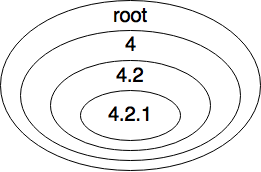
\includegraphics[width=2.5in]{idagent.png} 
   \caption{Identificador de un agente}
   \label{fig:agentid}
\end{figure}

%% Secci\'on:  %%
\section{Modelamiento formal de los operadores}
\label{syntax.rew}

Los operadores descritos en la Definici\'on~\ref{def:gensyn} est\'an representados por el sort \cde{SCCPCmd} en el modulo funcional \cde{SCCP-SYNTAX} tal como se muestra a continuaci\'on:

\begin{maude}
  sort SCCPCmd .

  op 0 : -> SCCPCmd . 
  op tell_ : Boolean -> SCCPCmd . 
  op ask_->_ : Boolean SCCPCmd -> SCCPCmd .
  op ask<_>_->_ : Aid Boolean SCCPCmd -> SCCPCmd .
  op _||_ : SCCPCmd SCCPCmd -> SCCPCmd [assoc gather (e E) ] .
  op <_>[_] : Aid SCCPCmd -> SCCPCmd .
\end{maude}

El argumento del operador \cde{tell_} es la restricci\'on o informaci\'on que se va a adicionar al banco de un agente, representado por un elemento de tipo \cde{Boolean}. El operador \cde{ask_->_} tiene como argumentos la condici\'on a ser evaluada dentro del banco de informaci\'on del agente y el proceso a llevarse a cabo. Cada uno de estos argumentos esta representado por elementos del tipo \cde{Boolean} y \cde{SCCPCmd}, respectivamente.

El operador \cde{ask_->_} permite verificar la satisfacibilidad de la restricci\'on dentro del banco de informaci\'on de un agente, en este modelo se presenta una extensi\'on a este operador mediante la cual se puede verificar la satisfacibilidad de la restricci\'on en un agente de menor jerarqu\'ia (i.e. el agente con \cde{ID} 4 puede preguntar al agente con \cde{ID} 4.2 o 2.3.1). Este operador esta definido como \cde{ask<_>_->_} y adicionalmente tiene como operador el identificador del agente de menor jerarqu\'ia, representado por un elemento de tipo \cde{Aid}.

El operador \cde{_||_} tiene como argumentos los procesos que se van a ejecutar en paralelo, representados por elementos de tipo \cde{Aid}. Finalmente, los argumentos del operador \cde{<_>[_]} son el identificador del agente y el proceso a ejecutar, representados por elementos del tipo \cde{Aid} y \cde{SCCPCmd}, respectivamente. 

%% Secci\'on:  %%
\section{Modelamiento formal de agentes y procesos}
\label{state.rew}

Los agentes y procesos est\'an representados como objetos por el sort \cde{Obj} definido en el modulo funcional \cde{SCCP-STATE} de la siguiente manera:

\begin{maude}
  sorts Cid Obj Cnf Sys .
  subsorts Obj < Cnf .
  
  ops store process : -> Cid .
  op [_,_,_] : Cid Aid Boolean -> Obj [ctor] .
  op [_,_,_] : Cid Aid SCCPCmd -> Obj [ctor] .
  op mt : -> Cnf [ctor] .
  op __ : Cnf Cnf -> Cnf [ctor assoc comm id: mt] .
  op {_} : Cnf -> Sys [ctor] .
\end{maude}

El sort \cde{Cid} representa el identificador de clase, en este caso agentes y procesos designados como \cde{store} y \cde{process}, respectivamente. Un agente esta representado como objeto de la forma \cde{[_,_,_]} cuyos argumentos son el identificador de clase (i.e. \cde{store}), el identificador del agente y su banco de informaci\'on. Cada uno de estos argumentos est\'an representados por elementos del tipo \cde{Cid}, \cde{Aid} y \cde{Boolean}, respectivamente.

Los argumentos de un proceso son el identificador de clase (i.e. \cde{process}), el identificador del agente y el proceso a ejecutar dentro del espacio de dicho agente. Estos argumentos est\'an representados por elementos del tipo \cde{Cid}, \cde{Aid} y \cde{SCCPCmd}, respectivamente.

Los estados del sistema est\'an representados por el sort \cde{Sys} definido como una sopa de agentes y procesos, dicha sopa es conmutativa, asociativa y tiene un elemento identidad. En la sintaxis de Maude, estos atributos se agregan incluyendo las palabras clave \cde{assoc}, \cde{comm} y \cde{id} en la declaraci\'on de las operaciones. El elemento identidad es \cde{mt}.

%% Secci\'on:  %%
\section{Modelamiento formal de las transiciones}
\label{rules.rew}

Las transiciones concurrentes del sistema est\'an modeladas por seis reglas de reescritura en la sintaxis de Maude, que corresponden a los operadores descritos en la Secci\'on~\ref{syntax.rew}. En las transiciones los procesos se ejecutan y los agentes cambian su banco de informaci\'on. Las reglas de reescritura se especifican a continuaci\'on: 

\begin{maude}
  rl [tell] :
     { [ store, L, B] [process, L, tell B0 ] X }
  => { [ process, L, 0 ] [ store, L, B and B0] X } .

 crl [ask] :
     { [ store, L, B ] [ process, L, ask B0  -> C0 ] X }
  => { [ store, L, B ] [ process, L, C0 ] X }
  if check-unsat(B and not(B0)) .

 crl [ask-ext0] :
     { [ store, L0 . L1, B ] 
       [ process, L0, ask< L1 > B0  -> C0 ] X }
  => { [ store, L0 . L1, B ] [ process, L0, C0 ] X }
  if check-unsat(B and not(B0)) . 

 crl [ext-ask1] :
     { [ process, L0, ask< L1 > B0  -> C0 ] X }
  => { [ process, L0, C0 ] X }
  if exists-store?(X, L0 . L1) == false
  /\ check-unsat(not(B0)) . 

  rl [parallel] :
     { [ process, L, C0 || C1 ] X }
  => { [ process, L, 0 ] [ process, L, C0 ] 
       [ process, L, C1 ] X } .

  rl [space] :
     { [ process, L0, < L1 >[ C0 ] ] X } 
  => { [ process, L0, 0 ] [ process, L0 . L1, C0] 
       [ store, L0 . L1, true ] X } .
\end{maude}

Las reglas \cde{[ask]}, \cde{[ask-ext0]} y \cde{[ext-ask1]} son condicionales, es decir, requieren que una condici\'on especifica se cumpla para poder ser ejecutadas, dicha condici\'on debe ser de tipo \cde{Boolean}.

Adicionalmente, se incluyen dos ecuaciones correspondientes a transiciones concurrentes no observables. La primer ecuaci\'on reemplaza un proceso inactivo (i.e. que no hace nada) por el elemento identidad del sistema \cde{mt}, y la segunda ecuaci\'on une dos agentes con el mismo identificador mediante una conjunci\'on l\'ogica de sus bancos de informaci\'on. Estas ecuaciones se especifican a continuaci\'on:

\begin{maude}
  eq [ process, L, 0 ]
   = mt .
  eq [ store, L, B0 ] [ store, L, B1 ]
   = [ store, L, B0 and B1 ] .
\end{maude}

%% Secci\'on:  %%
\section{Ejemplo}
\label{example.rew}

Esta secci\'on muestra c\'omo evoluciona el sistema usando la especificaci\'on de los operadores en la Secci\'on~\ref{syntax.rew}, los agentes y procesos en la Secci\'on~\ref{state.rew} y las reglas de reescritura de la Secci\'on~\ref{rules.rew}.

Considere el ejemplo del Capitulo~\ref{chapter.sccp}, el estado inicial $d$ puede ser escrito de la siguiente manera:

\begin{maude}
{ [store, root, (V:Integer > 10)]
  [store, 1, (W:Integer === 3)]
  [store, 1 . 3, (X:Integer === 17)]
  [store, 2, (Y:Integer > 4)]
  [store, 2 . 1, (Z:Integer === 20)] } 
\end{maude}

Los procesos $R$, $P$ y $Q$ se definen como,

\begin{maude}
[process, 1, ((< 3 >[tell(V:Integer === 42)]) || 
              (tell (T:Integer === 8)))]
[process, 2, (ask(Y:Integer > 0) -> tell(Z:Integer > 10))]
[process, 1, (ask(T:Integer > 7) -> 
              < 2 >[tell(S:Integer =/== 2)])]
\end{maude}

Por lo tanto, el proceso $S = \sfunc{R}_1 \parallel \sfunc{ P }_2 \parallel \sfunc{ Q }_1$ puede ser escrito as\'i:

\begin{maude}
[process, root, (((< 1 >[(< 3 >[tell(V:Integer === 42)]) || 
  (tell (T:Integer === 8))]) || 
  (< 2 >[ask(Y:Integer > 0) -> tell(Z:Integer > 10)])) || 
  (< 1 >[ask(T:Integer > 7) -> < 2 >[tell(S:Integer =/== 2)]]))]
\end{maude}

Al ejecutar el proceso junto con el estado inicial del sistema en el ambiente de Maude mediante el comando \cde{rew}, se obtiene el estado final del sistema, que debe 

\begin{maude}
rew { [store, root, (V:Integer > 10)]
  [store, 1, (W:Integer === 3)]
  [store, 1 . 3, (X:Integer === 17)]
  [store, 2, (Y:Integer > 4)]
  [store, 2 . 1, (Z:Integer === 20)]
  [process, root, (((< 1 >[(< 3 >[tell(V:Integer === 42)]) || 
     (tell (T:Integer === 8))]) || 
     (< 2 >[ask(Y:Integer > 0) -> tell(Z:Integer > 10)])) || 
     (< 1 >[ask(T:Integer > 7) -> 
      < 2 >[tell(S:Integer =/== 2)]]))] } .
\end{maude}

~\ref{fig:sccptree2}

\begin{maude}
{ [store,root,V:Integer > (10).Integer]
  [store,(1).NzNat,W:Integer === (3).Integer 
           and T:Integer === (8).Integer] 
  [store,(2).NzNat,Y:Integer > (4).Integer 
           and Z:Integer > (10).Integer] 
  [store,1 . 2,S:Integer =/== (2).Integer] 
  [store,1 . 3,X:Integer === (17).Integer 
           and V:Integer === (42).Integer] 
  [store,2 . 1,Z:Integer === (20).Integer] }
\end{maude}


